\chapter{State of the art}
This chapter will go through relevant articles and already known knowledge on the subject of mixed criticality systems. It will also explain the EMC2DP.

\section{Mixed criticality systems}
%SotA regarding MCS.
A MCS is achieved by letting applications of different criticality share resources. These resources could be the processor, memory, peripherals, input/output ports etc. The most explored area is sharing the CPU between multiple criticality levels \cite{burns2016}. The benefit of combining previously distributed systems is higher resource efficiency, which leads to economical benefits.\\

%The term Mixed Criticality had been used before 2007 to address issues of non-interference in non-federated architectures such as IMA [190];

\subsection{Economical benefits of MCS}
%Lower production cost, higher design cost?
Potential benefits with pursuing MCS as opposed to distributed systems are reduced physical space required, reduced weight, reduced heat generation, reduced power consumption and reduced production costs~\cite{burns2016}. This would all ultimately lead to economical benefits.\\

Potential downsides are increased complexity which could lead to higher system design costs. Building applications on the same platform to share resources could require engineering teams to work more closely together, potentially leading to administrative difficulties and costs. This needs to be investigated and could vary from industry to industry. To combat the potential downsides, the EMC\textsuperscript{2} project aims at creating platforms for easier development of MCS.\\ %TODO: källa eller ändra wording

The EMC\textsuperscript{2} project lists several goals \cite{website:emc2goals}:
\begin{itemize}
\item Reduce the cost of the system design by 15\%
\item Reduce the effort and time required for re-validation and re-certification of systems after making changes by 15\%
\item Manage a complexity increase of 25\% with 10\% effort reduction
\item Achieve cross-sectorial reusability of Embedded Systems devices and architecture platforms that will be developed using the ARTEMIS JU results.
\end{itemize}

\subsection{Sharing processor}
%A lot of work has been done regarding processor scheduling in MCS
%TODO: Wording
To deal with many different tasks needing processor time, different schedulers can be used to appropriately distribute processor time among the tasks.

\subsubsection{Conventional scheduling}
Fixed priority
Deadline monotonic
Rate monotonic
Earliest deadline first
Round robin

\subsubsection{Mixed criticality scheduling}
The area of sharing the processor in MCS was first explored by Steve Vestal~\cite{vestal2007} in 2007. His paper showed that neither Rate Monotonic (RM) nor Deadline Monotonic (DM) priority assignment was optimal for MCS; however Audsley’s optimal priority assignment algorithm \cite{audsley2001} was found to be applicable. \\ %TODO: Wording

In 2008 Baruah and Vestal~\cite{baruah2008} showed that EDF (Earliest Deadline First) does not dominate FP when criticality levels are introduced, and that there are feasible systems that cannot be scheduled by EDF.

%Schedulers
1. (audsley)~\cite{audsley2001} 2. EDF-VDL 3. SMC 4. AMC-max 5. AMC-rtb \cite{baruah2011}

"This figure plots the percentage of task sets generated that were deemed schedulable for a system of 20 tasks, with on average 50\% of those tasks having high criticality and each task having a high criticality execution time that is twice its low criticality execution time. The compared approaches are (from least effective to most effective): CrMPO which assigned priorities in criticality order, SMC-NO (static  mixed criticality with no run-time  monitoring) which  is  Vestal’s  original approach, SMC which is an adaptation of Vestal’s approach in which LO-criticality tasks are monitored at run-time and are prevented from executing for more than C(LO), and AMC-rtb and AMC-max which are the two methods introduced in the previous paragraph (AMC for adaptive mixed criticality). In the graph the UB-H\&L line bounds the maximum possible number of schedulable task sets. It serves to illustrate the quality of the AMC-max approach."~\cite{burns2016}

\begin{figure}[H]
\centering
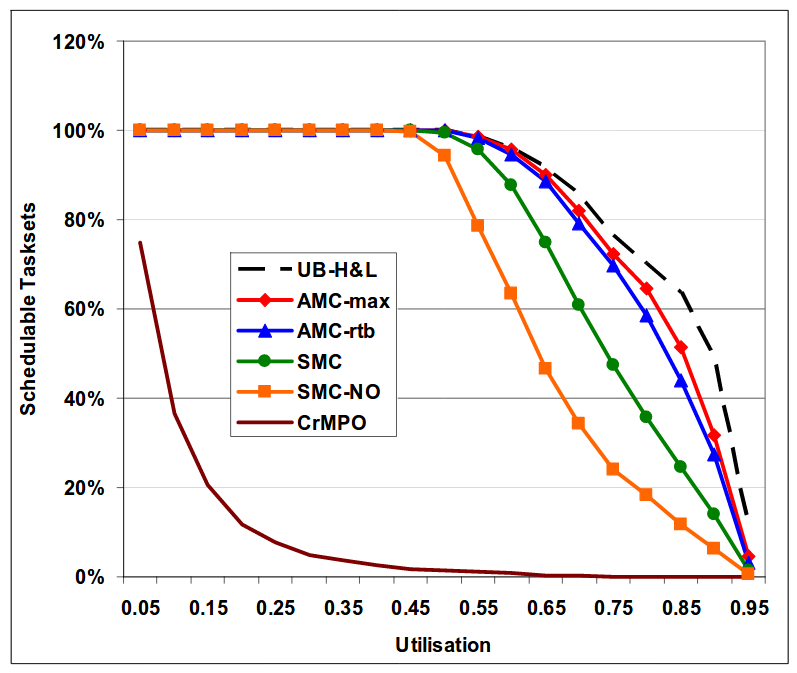
\includegraphics[width=\textwidth]{./img/literature_schedulers.png}
\caption{Percentage of schedulable tasks.~\cite{baruah2011}}\label{fig:schedulers}
\end{figure}

For a more complete review of work done on MCSs with a shared processor, see the paper by Burns~\cite{burns2016}.

\subsection{Different criticality on different processors}


\subsection{Sharing memory}
%http://pertsserver.cs.uiuc.edu/~mcaccamo/papers/euromicro12.pdf

\section{Current system}
\label{sec:lit_emc2mcs}
%TODO: bättre rubrik
%Describe current system more in depth.
This section will describe the EMC2DP, for more information see the report by Zaki~\cite{zaki2016}.

\subsection{Hardware}
The Zynq-7000 SoC has a Processing System (PS) consisting of a hardwired application processing unit, memory controller, and peripheral devices. The main processing unit is a dual-core Cortex-A9 ARM processor. Connected to the PS region is a Programmable Logic (PL) region. The PL is based on Xilinx’s 7-series FPGA technology. 
Due to the flexible nature of the PL, systems can be designed to reach a new level of performance. For example, the PL region can be used to instantiate standard or custom IP hardware modules that can serve as accelerators for the PS. Additionally, the PL region enables the PS to access system resources that are only accessible by the PL. %TODO: Wording
An overview of the interfaces between the PS and the PL can be seen in Figure~\ref{fig:interface}.\\ 

\begin{figure}[H]
\centering
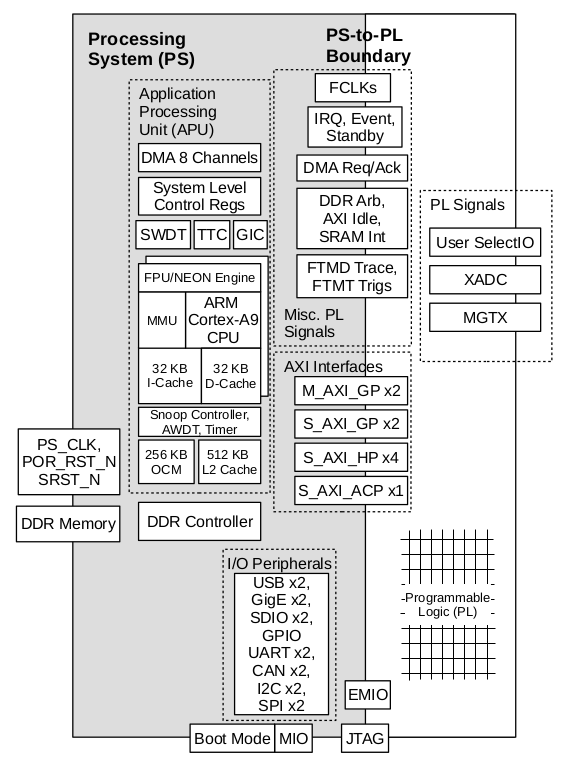
\includegraphics[width=0.5\textwidth]{./img/literature_interface.png}
\caption{Overview of the interfaces between the PS and PL regions.\cite{zaki2016}}\label{fig:interface}
\end{figure}

The interfaces between the PS and PL regions can be divided into two categories: 
\begin{itemize}
\item Functional interfaces: include the Advanced eXtensible Interface (AXI) ports such as AXIGP for general purpose master/slave device interface between PS and PL regions, extended MIO (EMIO) which enable PL IPs to access most I/O peripherals, interrupts, DMA flow control, clocks, and debug interfaces.
\item Configuration interfaces: these signals are connected to the configuration block of the PL, which allow the PS to control the configuration of the PL. %TODO: Wording
\end{itemize}

Resources are separated as secure and non-secure using ARM TrustZone \cite{website:ARM}.\\

\subsection{TrustZone}
\label{sec:trustzone}
TrustZone is a security feature by ARM that is available in their modern processors. TrustZone creates a security infrastructure in order to protect critical system assets from beeing accessed by non-trusted sources. This is achieved by enabling partitioning system components, both hardware and software, into either a Secure or Normal zone. Resources that are marked as Normal are not permitted to access Secure resources. This mechanism is enforced by the AMBA3 (Advanced Microcontroller Bus Architecture) AXI bus system. It contains an extra control signal for each of the read and write channels that dictate the access rights Non-secure bus masters to the Secure slaves. Each processor with an enabled TrustZone security extension can be partitioned into a Normal and a Secure virtual CPU. The virtual processors execute in a time-multiplexed fashion, and use the ”Monitor Mode” state to create an efficiently switching mechanism between Normal and Secure zones.~\cite{zaki2016} \\ %TODO: Wording

\subsection{Operative systems}
The EMC2DP uses two Operative Systems (OS) to create temporal and spatial separation between safety-critical and non-critical applications using TrustZone. In its current setup the Real-Time Operative System (RTOS) FMP by TOPPERS~\cite{website:FMP} is used for safety-critical applications. This RTOS follows the uITRON4.0 specification~\cite{uitron}, which is a widely used RTOS specification for Japanese embedded systems. For non-critical applications, the General Purpose Operative System (GPOS) Linux kernel 4.4 is used. Instead of Linux another instance of FMP could be used for non-critical applications.\\

\subsection{Virtual Machine Monitor}
A Virtual Machine Monitor (VMM) or "Hypervisor" is used to alternate between the safety-critical and non-critical OS. The VMM used is SafeG \cite{website:safeg}, also developed by TOPPERS. It switches processor state via a hardware switch. See figure~\ref{fig:modeswitch}. The switching takes ~2 $\mu s$.

\begin{figure}[H]
\centering
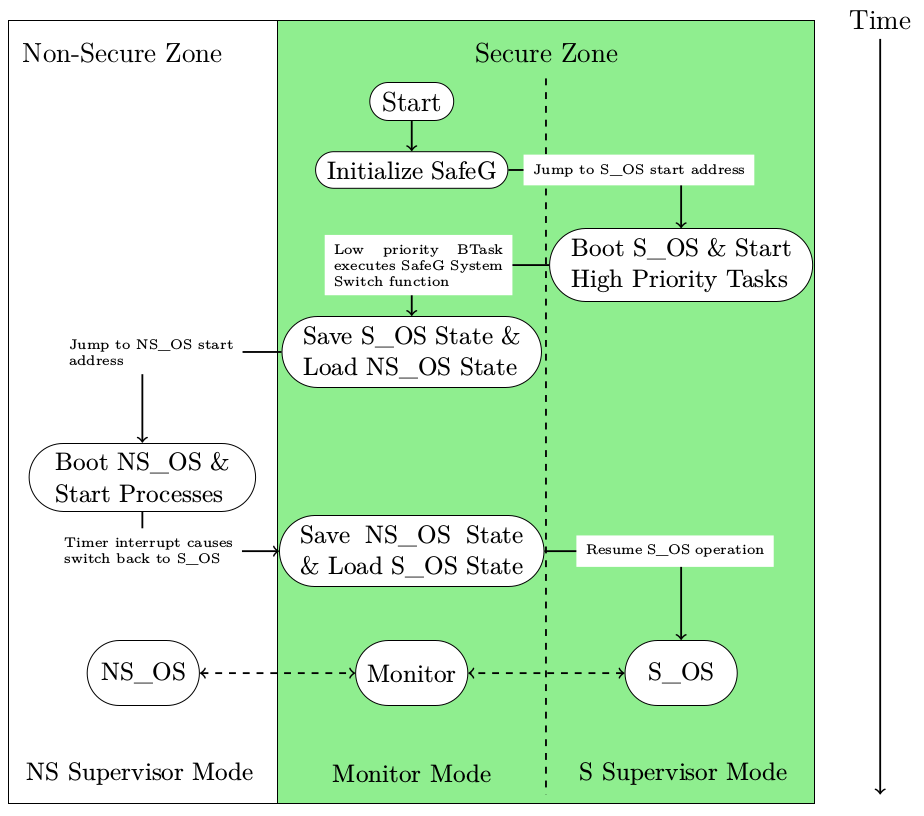
\includegraphics[width=\textwidth]{./img/literature_modeswitch.png}
%Flowchart of how the physical CPU switches between the virtual CPUs
\caption{Flowchart of the boot sequence of the CPU. \cite{zaki2016}}\label{fig:modeswitch}
\end{figure}

An basic overview of the hardware and the software of the system can be seen in Figure~\ref{fig:system_overview}.

\begin{figure}[H]
\centering
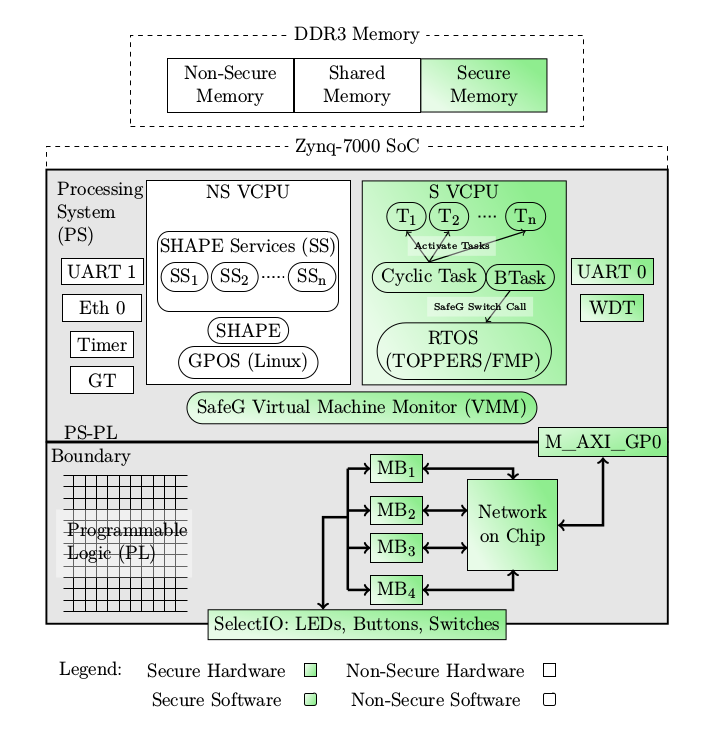
\includegraphics[width=\textwidth]{./img/literature_overview.png}
\caption{Overview of the MCS in place.\cite{zaki2016}}\label{fig:system_overview}
\end{figure}


\subsection{Build procedure}
The MCS is built from many different components. Hardware design,  applications, virtualization layer, operative systems, boot loaders etc. This section will describe the build procedure.\\ %TODO: Expand
%The virtualization layer (SafeG) and the Secure OS (RTOS) remain the same, the software that runs in the normal region can be either RTOS, GPOS, or a bare metal application. Furthermore, other configurations, such as RTOS or GPOS only mode, do not include the VMM.

Xilinx's software Vivado~\cite{website:vivado} is used to synthesize the hardware design (vhdl or verilog code) into a bitstream file (.bit) in order to configure the PL region of the Zynq. Vivado also produces a set of files that represent the designed hardware platform, which are used for software development. Xilinx SDK tool is used to create the Board Support Package (BSP) and the First Stage Boot Loader (FSBL) that correspond to the designed system. The FSBL is an Executable and Linkable Format (ELF) file that contains initialization software. During system boot, the FSBL is loaded into the On-Chip Memory (OCM) in order to initialize all available components (e.g. memory controller, data cache, instruction cache). In general, after the FSBL initialization process completes, and depending on boot sequence, the CPU can do any of the following actions: configure the FPGA, initiate the Second Stage Boot Loader SSBL, or jumps to the first address of the main program. The SDK tool is also used to generate a boot file (BOOT.bin), which must at least contain the FSBL (fsbl.elf). In the implemented system, the BOOT.bin file also includes the bitstream file (system.bit) and the SSBL (uboot.elf * ) The u-boot.elf file (universal boot-loader) is the SSBL. Once the system is initialized and the PL is configured, the system starts executing the u-boot instructions present in the BOOT.bin. U-boot is a full system on its own, and has many useful features. In particular, u-boot can be used to load executables and other system files from a remote server into the DDR3 memory using protocols such as Trivial File Transfer Protocol (TFTP) (Figure 6.3). This method is extremely usefully, particularly when dealing with large files during the development phase, such as the Root File System and Linux kernel.

Figure \ref{fig:system_build} provides a summary of the different dependencies for the system and the required flow for building the system. The keyword ”step x” indicates instances where dependencies exists within a build directory. Software tools are indicated by the circular shape, such as Vivado, SDK, and GNU Compiler Collection (GCC) (make).

\begin{figure}[H]
\centering
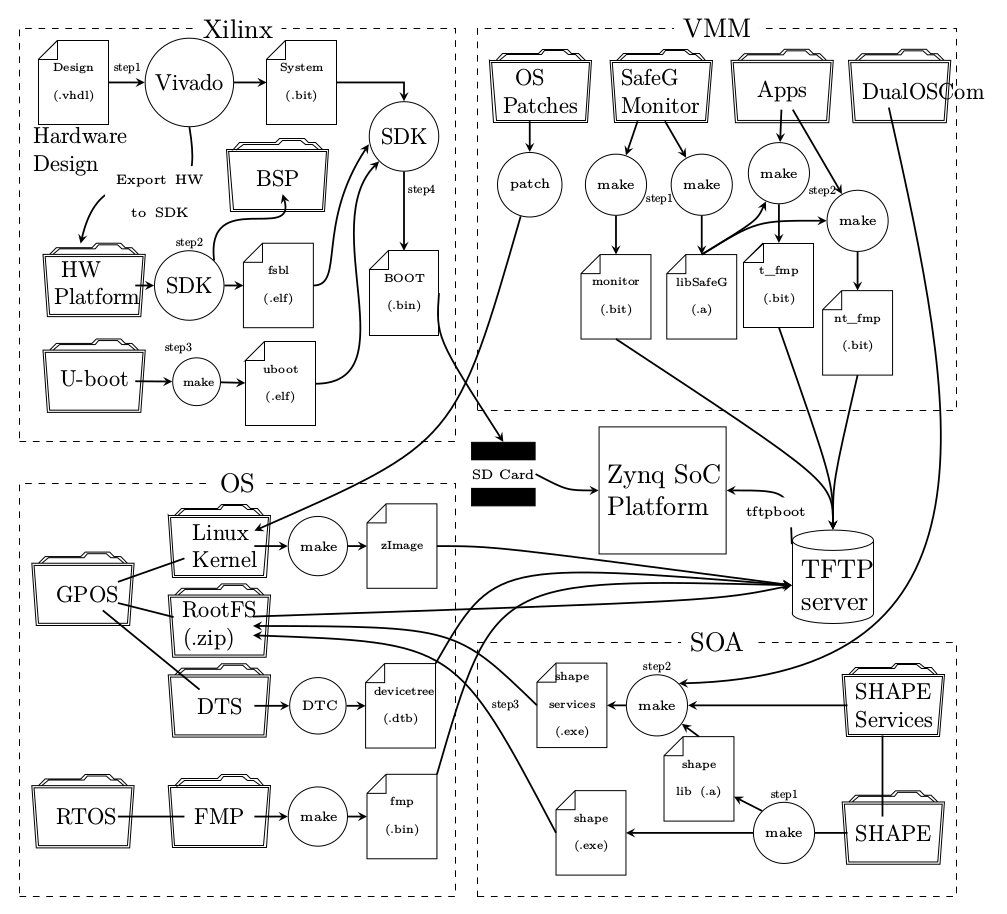
\includegraphics[width=\textwidth]{./img/literature_build.png}
\caption{System build procedure.\cite{zaki2016}}\label{fig:system_build}
\end{figure}

For more information about the build and the system, see the report by Zaki~\cite{zaki2016}.

\section{Standards}
%Different standards to regulate and ensure safety
Safety practices are becoming more regulated as industries adopt a standardized set of practices for designing and testing products. %TODO: expand, wording

\subsection{IEC 61508}
IEC 61508~\cite{IEC61508} is intended to be a basic functional safety standard for electrical and electronic systems applicable to all kinds of industry. It defines four different safety integrity levels, SIL~1 being the least dependable up to SIL~4 which is the most dependable level.

\subsection{ISO 26262}
ISO 26262~\cite{ISO26262} addresses the needs for an automotive-specific international standard that focuses on safety critical components. ISO 26262 is a derivative of IEC 61508.

\subsubsection{ASILs}
%ASIL QM (quality management) relates to the lowest (no) hazard, and ASIL
ISO 26262 describes five different Automotive Safety Integrity Levels (ASIL) relating to hazard and risk. Ranked from lowest (no) hazard to highest hazard, these levels are: QM, A, B, C and D. A function is assigned an ASIL depending on the severity if the function fails, the probability that the function fails and the controllability of the function, see table~\ref{table:ASIL}.

\begin{table}[H]
\centering
\begin{tabular}{|c|c|c|c|c|}
\hline
\multirow{2}{*}{\textbf{Severity}} &\multirow{2}{*}{\textbf{Probability}} &\multicolumn{3}{|c|}{\textbf{Controllability}} \\ \cline{3-5}
 & &C1 &C2 &C3 \\ \hline
\multirow{4}{*}{S1} & E1 & QM & QM & QM \\ \cline{2-5}
 & E2 & QM & QM & QM \\ \cline{2-5}
 & E3 & QM & QM & A \\ \cline{2-5}
 & E4 & QM & A & B \\ \hline
\multirow{4}{*}{S2} & E1 & QM & QM & QM \\ \cline{2-5}
 & E2 & QM & QM & A \\ \cline{2-5}
 & E3 & QM & A & B \\ \cline{2-5}
 & E4 & A & B & C \\ \hline
\multirow{4}{*}{S3} & E1 & QM & QM & A \\ \cline{2-5}
 & E2 & QM & A & B \\ \cline{2-5}
 & E3 & A & B & C \\ \cline{2-5}
 & E4 & B & C & D \\ \hline
\end{tabular}
\caption{ASIL as a function of severity, probability and controllability.}
\label{table:ASIL}
\end{table}

The various integrity levels can be translated into integers (ASIL $QM = 0$; $A = 1$; $B = 2$; $C = 3$ and $D = 4$). If a hazard requires several components to fail, the added ASIL of these components is used to determine if there is an violation, assuming the components faults are statistically independent of each other. For example, a safety level ASIL B can be met by two independent components which each individually only meet ASIL A (and thus effectively $A + A = B$).~\cite{azevedo2014} \\ %TODO: semi Wording

The different ASILs relate to cost, see table~\ref{table:cost_heuritics}. %TODO: Expand, wording

\begin{table}[H]
\centering
\begin{tabular}{|c|c|c|c|c|c|}
\hline
\textbf{Cost Heuristic} & \textbf{QM} & \textbf{A} & \textbf{B} & \textbf{C} & \textbf{D} \\ \hline
Linear & 0 & 10 & 20 & 30 & 40 \\ \hline
Logarithmic & 0 & 10 & 100 & 1000 & 10000 \\ \hline
Experimental-I~\cite{azevedo2014} & 0 & 10 & 20 & 40 & 50 \\ \hline
Experimental-II~\cite{azevedo2014} & 0 & 20 & 30 & 45 & 55 \\ \hline
\end{tabular}
\caption{ASIL cost heuristics.}
\label{table:cost_heuritics}
\end{table}


\subsubsection{Freedom from interference}
%TODO: Källa, utveckla, wording
In ISO 26262, Part 1, Definition 1.49, freedom from interference is defined as: Absence of cascading failures between two or more elements that could lead to the violation of a safety requirement. 

element = "system or part of a system including components, hardware, software, hardware parts, and software units" (ISO 26262, Part 1, Definition 1.32)

cascading failure = "failure of an element of an item causing another element or elements of the same item to fail" (ISO 26262, Part 1, Definition 1.13)

\subsection{AUTOSAR}
%TODO: Wording
"AUTOSAR (AUTomotive Open System ARchitecture) is a international development partnership of automotive interested parties founded in 2003. It pursues the objective of creating and establishing an open and standardized software architecture for automotive electronic control units (ECUs) excluding infotainment. Goals include the scalability to different vehicle and platform variants, transferability of software, the consideration of availability and safety requirements, a collaboration between various partners, sustainable utilization of natural resources, maintainability throughout the whole "Product Life Cycle"."~\cite{website:autosar}

The AUTOSAR Architecture distinguishes on the highest abstraction level between three software layers: Application, Runtime Environment (RTE) and Basic Software (BSW) which run on a Microcontroller.~\cite{website:autosar} See figure \ref{fig:autosar}.
\begin{itemize}
\item The application software layer is mostly hardware independent.
\item The RTE represents the full interface for applications.
\item The BSW is divided in three major layers and Complex Drivers: Services, ECU Abstraction and Microcontroller Abstraction. Services are divided furthermore into functional groups representing the infrastructure for System, Memory and Communication Services.
\end{itemize}

\begin{figure}[H]
\centering
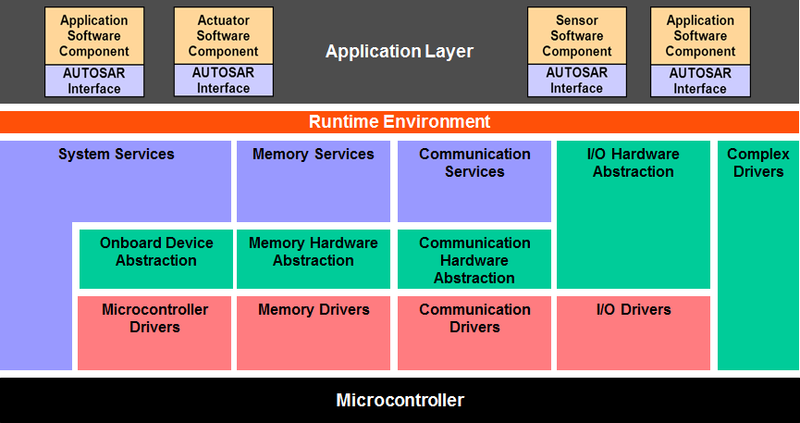
\includegraphics[width=\textwidth]{./img/literature_autosar.png}
\caption{AUTOSAR.~\cite{website:autosar}}\label{fig:autosar}
\end{figure}

